% Set the document class and theme
\documentclass[notheorems]{beamer}

\setbeamertemplate{theorem}[ams style]
\setbeamertemplate{theorems}[numbered]

\makeatletter
    \ifbeamer@countsect
      \newtheorem{theorem}{\translate{Theorem}}[section]
    \else
      \newtheorem{theorem}{\translate{Theorem}}
    \fi
    \newtheorem{corollary}{\translate{Corollary}}
    \newtheorem{fact}{\translate{Fact}}
    \newtheorem{lemma}{\translate{Lemma}}
    \newtheorem{problem}{\translate{Problem}}
    \newtheorem{solution}{\translate{Solution}}

    \theoremstyle{definition}
    \newtheorem{definition}{\translate{Definition}}
    \newtheorem{definitions}{\translate{Definitions}}

    \theoremstyle{example}
    \newtheorem{example}{\translate{Example}}
    \newtheorem{examples}{\translate{Examples}}

    % Compatibility
    \newenvironment{Lemma}{\begin{lemma}}{\end{lemma}}
    \newenvironment{Proof}{\begin{proof}}{\end{proof}}
    \newenvironment{Theorem}{\begin{theorem}}{\end{theorem}}
    \newenvironment{Problem}{\begin{problem}}{\end{problem}}
    \newenvironment{Corollary}{\begin{corollary}}{\end{corollary}}
    \newenvironment{Example}{\begin{example}}{\end{example}}
    \newenvironment{Examples}{\begin{examples}}{\end{examples}}
    \newenvironment{Definition}{\begin{definition}}{\end{definition}}
\makeatother

\usetheme{Madrid}
\useoutertheme{miniframes} % Alternatively: miniframes, infolines, split
\useinnertheme{circles}

\definecolor{IITHorange}{RGB}{243, 130, 33} % UBC Blue (primary)
\definecolor{IITHyellow}{RGB}{254, 203, 10} % UBC Grey (secondary)

\setbeamercolor{palette primary}{bg=IITHorange,fg=white}
\setbeamercolor{palette secondary}{bg=IITHorange,fg=white}
\setbeamercolor{palette tertiary}{bg=IITHorange,fg=white}
\setbeamercolor{palette quaternary}{bg=IITHorange,fg=white}
\setbeamercolor{structure}{fg=IITHorange} % itemize, enumerate, etc
\setbeamercolor{section in toc}{fg=IITHorange} % TOC sections

% Override palette coloring with secondary
\setbeamercolor{subsection in head/foot}{bg=IITHyellow,fg=white}

\setbeamertemplate{caption}[numbered]
\setbeamertemplate{theorems}[numbered]

\usepackage{./presentation_macros}

\title{The Retracing Boomerang Attack}
\subtitle{Orr Dunkelman, Nathan Keller, Eyal Ronen, and Adi Shamir\\EUROCRYPT 2020}
\author{Gautam Singh}
\institute[IITH]{Indian Institute of Technology Hyderabad}
\date{July 21, 2025}

\begin{document}
    
    \begin{frame}
        \titlepage
    \end{frame}
    
    \begin{frame}
        \tableofcontents[hideallsubsections]
    \end{frame}
    
    \section{Introduction}
    \label{sec:intro}
    
    \begin{frame}[<+->]{Introduction}
        \begin{enumerate}
            \item Broke the record for 5-round AES when it was
            published.
            \item Brings the attack complexity down to \(2^{16.5}\)
            encryptions.
            \item Uncovers a hidden relationship between boomerang attacks and
            two other cryptanalysis techniques: yoyo game and mixture
            differentials.
        \end{enumerate}
    \end{frame}

    \section{Preliminaries}
    \label{sec:prelims}

    \subsection{Boomerang Attacks}
    \label{subsec:boomerang}

    \begin{frame}{The Boomerang Attack}
        \begin{columns}
            \begin{column}{0.7\textwidth}
                \begin{enumerate}
                    \item<1-> Typically split the encryption function as \(E =
                    E_1 \circ E_0\), with differential trails for each
                    sub-cipher.
                    \item<2-> We can build a distinguisher that can distinguish
                    \(E\) from a truly random permutation in
                    \(\cO\brak{\brak{pq}^{-2}}\) plaintext pairs.
                \end{enumerate}
            \end{column}
            \begin{column}{0.3\textwidth}
                \begin{figure}[!ht]
                    \centering
                    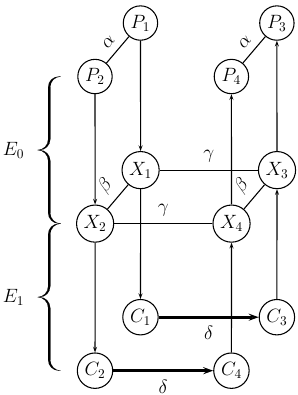
\includegraphics[width=\columnwidth]{images/boomerang.png}
                    \caption{The boomerang attack.}
                    \label{fig:boomerang}
                \end{figure}
            \end{column}
        \end{columns}
    \end{frame}

    \begin{frame}{The Boomerang Distinguisher}
        \begin{algorithm}[H]
            \caption{The Boomerang Attack Distinguisher}
            \label{alg:boomerang-dist}
            \algrenewcommand\alglinenumber[1]{\small ####1:}
            \small
            \begin{algorithmic}[1]
                \State Generate \(\brak{pq}^{-2}\) plaintext pairs \(\brak{P_1, P_2}\)
                such that \(P_1 \oplus P_2 = \alpha\).
                \ForAll {pairs \(\brak{P_1, P_2}\)}
                    \State Ask for the encryption of \(\brak{P_1, P_2}\) to \(\brak{C_1,
                    C_2}\).
                    \State Compute \(C_3 = C_1 \oplus \delta\) and \(C_4 = C_2 \oplus 
                    \delta\). \Comment{\(\delta\)-shift}
                    \State Ask for the decryption of \(\brak{C_3, C_4}\) to \(\brak{P_3,
                    P_4}\).
                    \If {\(P_3 \oplus P_4 = \alpha\)}
                        \State \Return This is the cipher \(E\)
                    \EndIf
                \EndFor
                \State \Return This is a random permutation
            \end{algorithmic}
        \end{algorithm}
    \end{frame}

    \subsection{The Yoyo Game}
    \label{subsec:yoyo-game}
    
    \begin{frame}[<+->]{The Yoyo Game}
        \begin{enumerate}
            \item Similar to boomerang, starts by encrypting \(\brak{P_1, P_2}\)
            to \(\brak{C_1, C_2}\), then modifying them to \(\brak{C_3, C_4}\)
            and decrypting them.
            \item Unlike the boomerang attack, this \emph{continues} in the yoyo
            game.
            \item All pairs of intermediate values \(\brak{X_{2l + 1}, X_{2l +
            2}}\) satisfy some property (such as zero difference in some part).
            \item Probabilities are low with large \(l\). Still, the yoyo
            technique has been used to attack AES reduced to 5 rounds.
        \end{enumerate}
    \end{frame}

    \subsection{Mixture Differentials}
    \label{subsec:mixture}
    
    \begin{frame}{Mixture}
        \begin{definition}[Mixture]
            \label{def:mixture}
            Suppose \(P_i \triangleq \brak{\rho_1^i, \rho_2^i, \ldots,
            \rho_t^i}\). Given a plaintext pair \(\brak{P_1, P_2}\), we say
            \(\brak{P_3, P_4}\) is a \emph{mixture counterpart} of \(\brak{P_1,
            P_2}\) if for each \(1 \le j \le t\), the quartet \(\brak{\rho_j^1,
            \rho_j^2, \rho_j^3, \rho_j^4}\) consists of two pairs of equal
            values or of four equal values. The quartet \(\brak{P_1, P_2, P_3,
            P_4}\) is called a \emph{mixture}.
        \end{definition}
        \pause
        \begin{enumerate}
            \item<2-> If \(\brak{P_1, P_2, P_3, P_4}\) is a mixture, then XOR of
            the intermediate values \(\brak{X_1, X_2, X_3, X_4}\) is zero.
            \item<3-> \(X_1 \oplus X_3 = \gamma \implies X_2 \oplus X_4 =
            \gamma\). Hence, for \(\gamma \xrightarrow{q} \delta\) in \(E_1\),
            \(C_1 \oplus C_3 = C_2 \oplus C_4 = \delta\) with probability
            \(q^2\).
        \end{enumerate}
    \end{frame}

    \begin{frame}{The SimpleSWAP Algorithm}
        \cref{alg:simple-swap} is a simple method to generate mixture
        counterparts.
        \begin{algorithm}[H]
            \caption{Swaps the first word where texts are different and returns one word.}
            \label{alg:simple-swap}
            \begin{algorithmic}[1]
                \Function{SimpleSWAP}{\(x^0\), \(x^1\)} \Comment{\(x^0 \ne x^1\)}
                    \State \(x^{\prime 0}, x^{\prime 1} \gets x^0, x^1\)
                    \For{\(i\) from 0 to 3}
                        \If{\(x_i^0 \ne x_i^1\)}
                            \State \(x_i^{\prime 0}, x_i^{\prime 1} \gets x_i^1, x_i^0\)
                            \State \Return \(x^{\prime 0}, x^{\prime 1}\)
                        \EndIf
                    \EndFor
                \EndFunction
            \end{algorithmic}
        \end{algorithm}
    \end{frame}

    \section[Retracing Boomerang Attack]{The Retracing Boomerang Attack}
    \label{sec:retr-boomerang}
    
    \subsection{The Retracing Boomerang Framework}
    \label{sec:retr-framework}

    \begin{frame}{The Retracing Boomerang Framework}
        \begin{figure}[!ht]
            \centering
            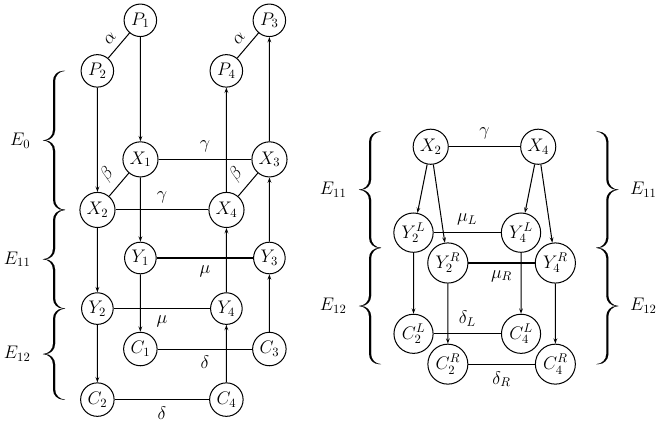
\includegraphics[width=0.6\columnwidth]{images/retracing_boomerang.png}
            \caption{The retracing boomerang attack.}
            \label{fig:retr-boomerang}
        \end{figure}
    \end{frame}

    \begin{frame}[<+->]{The Retracing Boomerang Attack}
        \begin{enumerate}
            \item The \emph{retracing boomerang} framework consists of a
            \emph{shifting} type and a \emph{mixing} type.
            \item Both attacks use the setup shown in \cref{fig:retr-boomerang}.
            \item Although the additional split looks restrictive, it applies
            for a wide class of block ciphers such as SASAS constructions.
            \item It is assumed that \(E_{12}\) can be split into two parts of
            size \(b\) and \(n - b\) bits, call these functions \(E_{12}^L\) and
            \(E_{12}^R\), with characteristic probabilities \(q_2^L\) and
            \(q_2^R\) respectively.
        \end{enumerate}
    \end{frame}

    \subsection{The Shifting Retracing Attack}
    \label{subsec:shift-retr-boomerang}

    \begin{frame}[<+->]{The Shifting Retracing Boomerang Attack}
        \begin{enumerate}
            \item Check if \(C_1^L \oplus C_2^L = 0 \textrm{ or } \delta_L\).
            \emph{Discard all pairs not satisfying this relation}. This is a
            \(\brak{b - 1}\)-bit filtering.
            \item \(\delta\)-shift is performed on the filtered ciphertext pairs
            to get \(\brak{C_3, C_4}\). This ensures \(\cbrak{C_1, C_3} =
            \cbrak{C_2, C_4}\).
            \item \emph{If one of these pairs satisfies \(\delta_L
            \xrightarrow{q_2^L} \mu_L\), the other pair will too!}. Increases
            the probability of the boomerang distinguisher by
            \(\brak{q_2^L}^{-1}\).
            \item Any possible characteristic of \(E_{12}^L\) has probability at
            least \(2^{-b + 1}\), thus overall probability increases by a factor
            of at most \(2^{b - 1}\). On the other hand, filtering only leaves
            \(2^{-b + 1}\) of the pairs, so \emph{no apparent gain?}
        \end{enumerate}
    \end{frame}

    \begin{frame}{The Shifting Retracing Boomerang Attack}
        \begin{figure}
            \centering
            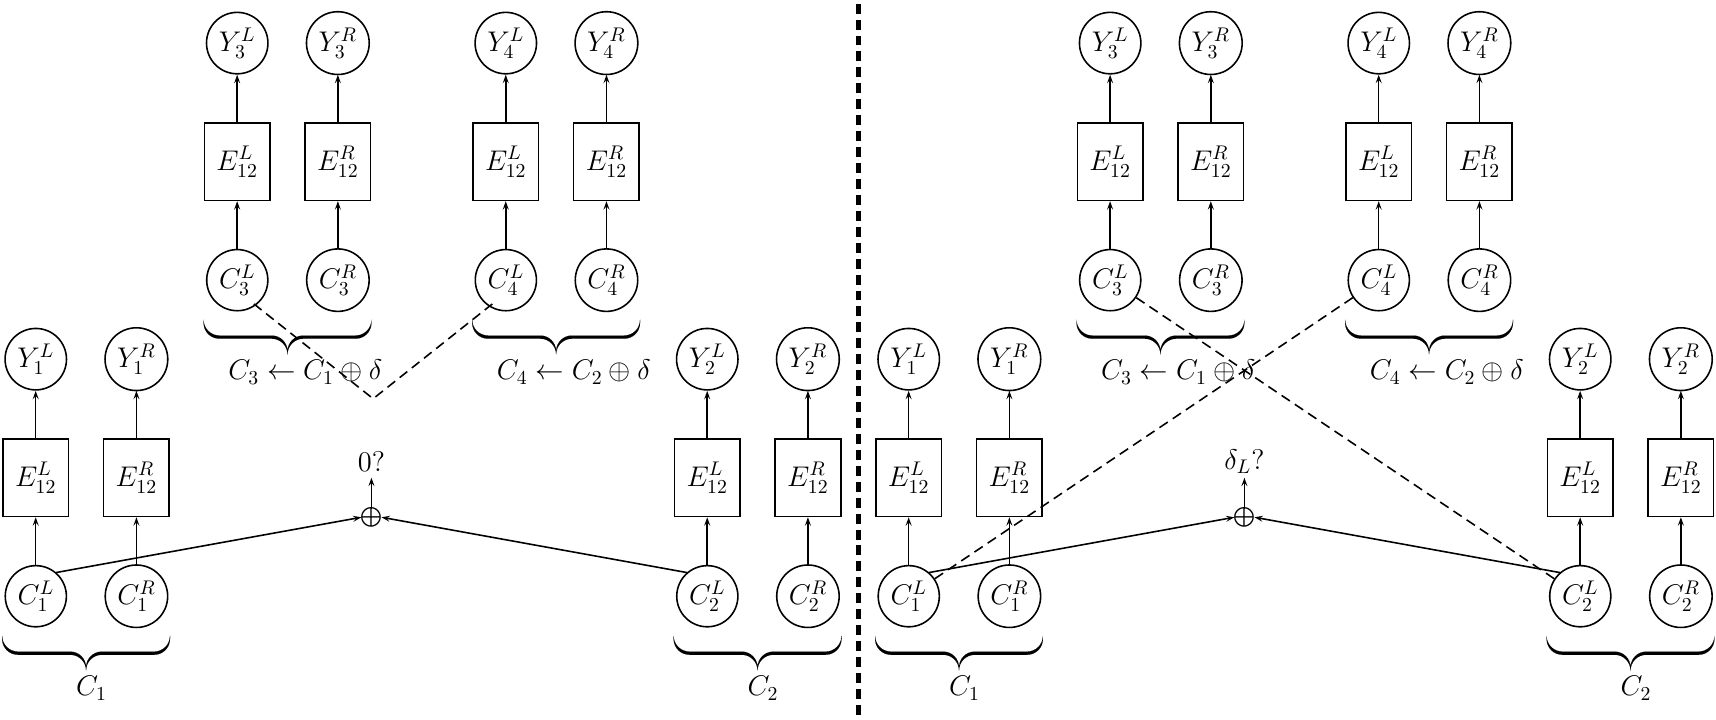
\includegraphics[width=\columnwidth]{images/shifting_boomerang.png}
            \caption{A shifted quartet (dashed lines indicate equality).}
        \end{figure}
    \end{frame}

    \subsection{The Mixing Retracing Attack}
    \label{subsec:mix-retr-boomerang}

    \begin{frame}[<+->]{The Mixing Retracing Boomerang Attack}
        \begin{enumerate}
            \item In shifting attack, \(\cbrak{C_1^L, C_2^L} = \cbrak{C_3^L,
            C_4^L}\) forced using a \(\delta\)-shift.
            \item Each ciphertext shifted by \(\brak{C_1^L \oplus C_2^L, 0}\),
            thus
            \begin{align}
                C_3 &= \brak{C_3^L, C_3^R} = \brak{C_1^L \oplus \brak{C_1^L \oplus C_2^L}, C_1^R} = \brak{C_2^L, C_1^R}, \\
                C_4 &= \brak{C_4^L, C_4^R} = \brak{C_2^L \oplus \brak{C_1^L \oplus C_2^L}, C_2^R} = \brak{C_1^L, C_2^R}.
            \end{align}
            Here, \(\cbrak{C_1^L, C_2^L} = \cbrak{C_3^L, C_4^L}\).
            \item Further, \(C_1^R = C_3^R\) and \(C_2^R = C_4^R\).
            \emph{Additional} gain of \(\brak{q_2^R}^{-2}\) for total
            probability \(\brak{pq_1}^2q_2^L\), \emph{better than shifting!}
            \item Similar to the core step used in the yoyo attack on AES.
        \end{enumerate}
    \end{frame}

    \begin{frame}{The Mixing Retracing Boomerang Attack}
        \begin{figure}
            \centering
            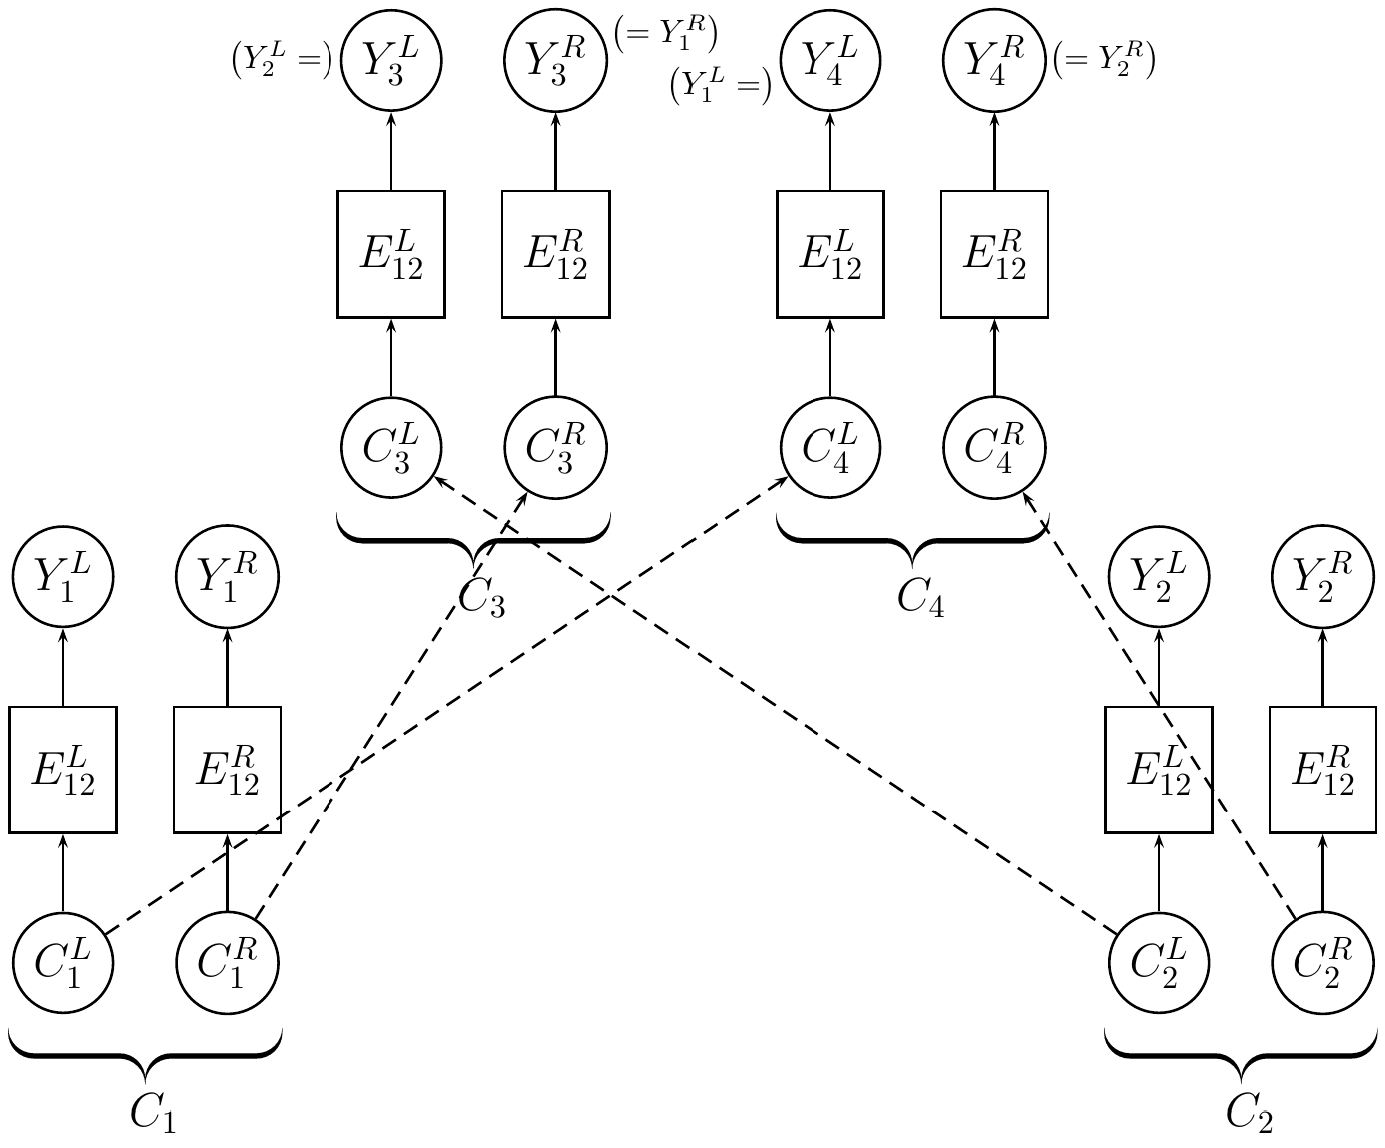
\includegraphics[width=0.55\columnwidth]{images/mixing_boomerang.png}
            \caption{A mixture quartet of ciphertexts (dashed lines indicate equality).}
        \end{figure}
    \end{frame}

    \subsection{Comparison Between the Two Types of Retracing Attacks}
    \label{subsec:cmp}
    \begin{frame}[<+->]{Advantages of Shifting Retracing Attack}
        \begin{enumerate}
            \item \textbf{Using structures}
            \begin{itemize}[<+->]
                \item Shifting applies the same \(\delta\)-shift to all pairs of
                ciphertexts.
                \item Filtering applied first reduces the data complexity. No
                filtering in mixing since shift is based on ciphertexts.
                \item With shifting, one can obtain all ciphertexts, shift them
                by \(\delta\) and then decrypt, simultaneously checking for the
                filter and condition between \(P_3\) and \(P_4\) using a hash
                table.
            \end{itemize}
            \item \textbf{Combination with \(E_{11}\)}
            \begin{itemize}[<+->]
                \item In mixing, the output difference of \(E_{12}^L\) is
                arbitrary.
                \item Usually no good combination between characteristics of
                \(\brak{E_{12}^L}^{-1}\) and \(\brak{E_{11}}^{-1}\). For
                instance, in the yoyo attack, \(E_{11}\) is empty.
            \end{itemize}
            \item \textbf{Construction of `friend pairs'}
            \begin{itemize}[<+->]
                \item `Friend pairs' are pairs which satisfy a common property.
                \item More `friend pairs' can be constructed in the shifting
                variant.
            \end{itemize}
        \end{enumerate}
    \end{frame}

    \section[Application to AES]{Retracing Boomerang Attack on Five Round AES}
    \label{sec:retr-boomerang-aes}

    \subsection{Brief Description of AES}
    \label{subsec:aes-description}

    \begin{frame}{Description of AES}
        \begin{enumerate}[<+->]
            \item Byte ordering shown after \(SB\) in \cref{fig:aes} (column
            major).
            \item \(j\)-th byte of a state \(X_i\) is denoted as \(X_{i,j}\) or
            \(\brak{X_i}_j\).
            \item Denote by \(W, Z\) and \(X\) the states before \(MC\) in round
            0, at the input to round 1 and before \(MC\) in round 2
            respectively.
            \item The \(l\)-th shifted column (resp. \(l\)-th inverse shifted
            column) refers to application of \(SR\) (resp. \(SR^{-1}\)) to the
            \(l\)-th column.
            \item Round subkeys are \(k_{-1}, k_0, \ldots\).
        \end{enumerate}
        \begin{figure}[!ht]
            \centering
            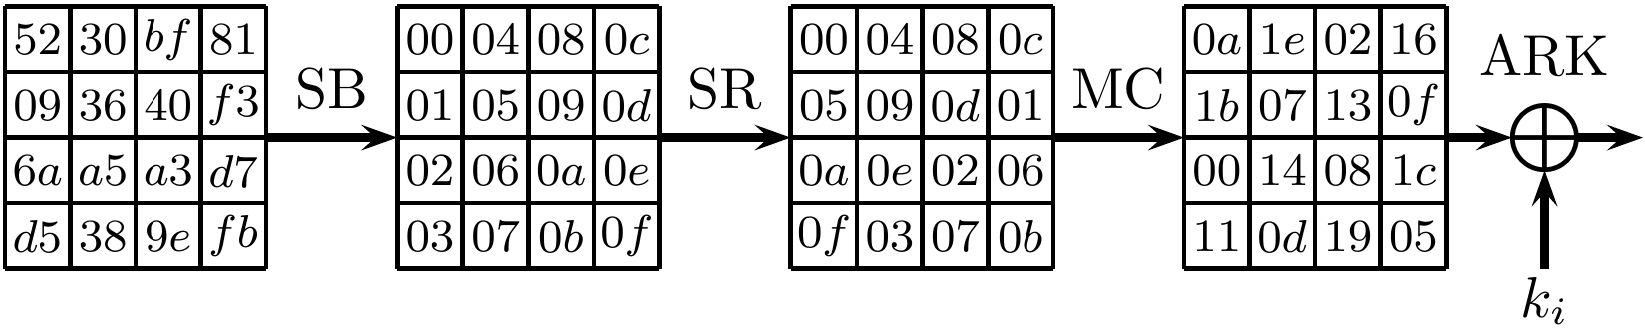
\includegraphics[width=0.85\columnwidth]{images/aes.png}
            \caption{An AES round.}
            \label{fig:aes}
        \end{figure}
    \end{frame}

    \subsection{The Yoyo Attack on Five Round AES}
    \label{subsec:yoyo-aes}

    \begin{frame}[<+->]{Summary of Yoyo Attack on Five Round AES}
        \begin{enumerate}
            \item Decomposes AES as \(E = E_{12} \circ E_{11} \circ E_0\) where
            \(E_0\) is the first 2.5 rounds, \(E_{11}\) is the MC of round 2 and
            \(E_{12}\) is the last 2 rounds.
            \item Truncated differential characteristic for \(E_0\): zero input
            difference in three inverse shifted columns and zero output
            difference in a single shifted column with probability \(4 \cdot
            2^{-8} = 2^{-6}\).
            \item For \(E_{12}\), 1.5 rounds of AES can be taken as four 32-bit
            super S-boxes.
            \item Attack inverse shifted columns of \(k_{-1}\). Friend pairs
            used to get more information.
        \end{enumerate}
    \end{frame}

    \begin{frame}[<+->]{Meet in the Middle Improvement on Yoyo Attack}
        \begin{enumerate}
            \item Denote the value of byte \(m\) before \(MC\) operation of
            round 0 by \(W_m\), and WLOG let \(l = 0\). Then,
            \begin{equation}
                Z_0 = 02_x \cdot W_0 \oplus 03_x \cdot W_1 \oplus 01_x \cdot W_2 \oplus 01_x \cdot W_3.
                \label{eq:mitm}
            \end{equation}
            \item Adversary guesses \(k_{-1, \cbrak{0, 5}}\) by computing the
            following for \(j = 1, 2, 3\) and storing the concatenated 24-bit
            value in a hash table.
            \begin{equation}
                02_x \cdot \brak{\brak{W_3^j}_0 \oplus \brak{W_4^j}_0} \oplus 03_x \cdot \brak{\brak{W_3^j}_1 \oplus \brak{W_4^j}_1}
                \label{eq:mitm-0-5}
            \end{equation}
            \item We need \(Z_0 = 0\) to satisfy the truncated differential
            characteristic. Meet in the Middle (MITM) methods are used to narrow
            down candidates for \(k_{-1}\).
            \begin{itemize}
                \item Specific choice of plaintexts based on DDT of AES S-boxes.
                \item Eliminating key bytes using friend pairs.
            \end{itemize}
        \end{enumerate} 
    \end{frame}

    \begin{frame}[<+->]{Specific Choice of Plaintexts}
        \begin{enumerate}
            \item Choose plaintexts with non-zero difference \emph{only in bytes
            0 and 5.} Here, \(\brak{Z_1}_0 = \brak{Z_2}_0\) leaves \(2^8\)
            candidates for \(k_{-1, \cbrak{0, 5}}\), given by
            \begin{equation}
                02_x \cdot \brak{\brak{W_1}_0 \oplus \brak{W_2}_0} \oplus 03_x \cdot \brak{\brak{W_1}_1 \oplus \brak{W_2}_1} = 0.
                \label{eq:mitm-simple}
            \end{equation}
            \item Constrain \(\brak{P_1}_5 \oplus \brak{P_2}_5 = 01_x\) to
            detect right key bytes efficiently.
            \item DDT row of AES S-box for input difference \(01_x\) along with
            input pair(s) for each output difference computed and stored in
            memory.
            \item For each \(\brak{P_1, P_2}\) and for each guess of \(k_{-1,
            0}\), use \eqref{eq:mitm-simple} to compute the output difference of
            the SB operation in byte 5.
            \item Lookup to find inputs that can lead to this difference and
            retrieve possible values of \(k_{-1, 5}\) corresponding to the
            guessed \(k_{-1, 0}\).
            \item Obtain \(2^8\) candidates for \(k_{-1, \cbrak{0, 5}}\) in
            about \(2^8\) operations per pair.
        \end{enumerate}        
    \end{frame}

    \begin{frame}[<+->]{Eliminating Key Bytes Using Friend Pairs}
        \begin{enumerate}
            \item To reduce the number of candidates for \(k_{-1, \cbrak{10,
            15}}\), the boomerang process is used to return multiple friend
            pairs \(\brak{P_3^j, P_4^j}\).
            \item In particular, we choose one such pair for which
            \begin{equation}
                \brak{P_3^j}_{10} \oplus \brak{P_4^j}_{10} = 0 \quad \textrm{or} \quad \brak{P_3^j}_{15} \oplus \brak{P_4^j}_{15} = 0.
                \label{eq:mitm-check}
            \end{equation}
            \item If equality holds in byte 10, then \(k_{-1, 15}\) is isolated
            for a fixed \(k_{-1, \cbrak{0, 5}}\) and has only \(2^8\) possible
            values.
            \item Requires \(2^9\) simple operations and leaves \(2^8\)
            candidates for \(k_{-1, \cbrak{0, 5, 15}}\).
            \item Similar MITM procedure followed with another friend pair to
            obtain the unique value of \(k_{-1, \cbrak{0, 5, 10, 15}}\) by
            isolating \(k_{-1, 10}\).
            \item Perform \(2^8\) operations for each pair \(\brak{P_1, P_2}\)
            and for each value of \(l\). Total time complexity of about
            \(2^{16}\) operations.
            \item Each pair requires \(2^7\) friend pairs to find one that
            satisfies \eqref{eq:mitm-check} with high probability. Total data
            complexity is increased to about \(2^{15}\).
        \end{enumerate} 
    \end{frame}

    \subsection{Attack Description and Analysis}
    \label{sec:retr-boomerang-algo}
    \begin{frame}[<+->]{Attack Algorithm}
        \begin{enumerate}
            \item \textbf{Precomputation:} Compute DDT row of AES S-box for
            input difference \(01_x\), along with actual inputs for each output
            difference.
            \item \textbf{Online Phase:} Take 64 pairs \(\brak{P_1, P_2}\) with
            \(\brak{P_1}_5 = 00_x\), \(\brak{P_2}_5 = 01_x\), \(\brak{P_1}_0 \ne
            \brak{P_2}_0\) and all other corresponding bytes equal.
            \item For each plaintext pair, create \(2^7\) friend pairs
            \(\brak{P_1^j, P_2^j}\) such that for each \(j\), \(P_1^j \oplus
            P_2^j = P_1 \oplus P_2\) and \(\brak{P_1^j}_{\cbrak{0, 5, 10, 15}} =
            \brak{P_1}_{\cbrak{0, 5, 10, 15}}\).
            \seti
        \end{enumerate}
    \end{frame}

    \begin{frame}[<+->]{Attack Algorithm}
        \begin{enumerate}
            \conti
            \item For each plaintext pair \(\brak{P_1, P_2}\) and for each \(l
            \in \cbrak{0, 1, 2, 3}\), do the following. (\(l = 0\) taken below)
            \begin{enumerate}[<+->]
                \item Use \eqref{eq:mitm-simple} to compute and store all
                \(2^8\) candidates for \(k_{-1, \cbrak{0, 5}}\) in a table.
                \item Use the boomerang process to obtain pairs \(\brak{P_3,
                P_4}\) and \(\brak{P_3^j, P_4^j}\).
                \item Find a \(j\) for which \eqref{eq:mitm-check} is satisfied.
                Perform an MITM attack on column 0 of round 0 using
                \(\brak{P_3^j, P_4^j}\) to obtain \(2^8\) candidates for
                \(k_{-1, \cbrak{0, 5, 15}}\).
                \item Perform another MITM attack on column 0 of round 0 using
                two plaintext pairs \(\brak{P_3^{j^\prime}, P_4^{j^\prime}}\).
                This gives a possible value for \(k_{-1, \cbrak{0, 5, 10,
                15}}\).
                \item If contradiction, go to the next value of \(l\). If
                contradiction for all \(l\), discard this pair and go to the
                next pair.
            \end{enumerate}
            \item Using a pair \(\brak{P_1, P_2}\) for which no contradiction
            occurred, perform MITM attacks on columns 1, 2 and 3 of round 0
            using the fact that \(Z_3 \oplus Z_4\) equals 0 in the \(l\)-th
            inverse shifted column to recover \(k_{-1}\). 
        \end{enumerate}
    \end{frame}

    \begin{frame}[<+->]{Attack Analysis}
        \begin{enumerate}
            \item Attack succeeds if data contains a pair that satisfies the
            truncated differential characteristic of \(E_0\) and if a friend
            pair has zero difference in either byte 10 or 15.
            \item Increasing the number of initial pairs and friend pairs per
            initial pair boosts success probability. With 64 pairs and 128
            friend pairs per initial pair, the probability of success is
            \(\brak{1 - e^{-1}}^2 \approx 0.4\)
            \item Another way to boost succees probability is to find other ways
            to cancel terms in \eqref{eq:mitm}. For instance, if there exist
            \(j, j^\prime\) such that \(\cbrak{\brak{P_3^j}_{10},
            \brak{P_4^j}_{10}} = \cbrak{\brak{P_3^{j^\prime}}_{10},
            \brak{P_4^{j^\prime}}_{10}}\), we can take the XOR of
            \eqref{eq:mitm} to cancel the effect of \(k_{-1, 10}\), thus
            increasing the success probability even when there is no pair that
            satisfies \eqref{eq:mitm-check}.
            \seti
        \end{enumerate} 
    \end{frame}

    \begin{frame}[<+->]{Attack Analysis}
        \begin{enumerate}
            \conti
            \item Data complexity is \(2 \cdot 2^6 \cdot 2^7 = 2^{14}\) chosen
            plaintexts and \(2^{14}\) adaptively chosen ciphertexts.
            \item Structures reduce the data complexity to slightly above
            \(2^{14}\) adaptively chosen ciphertexts and plaintexts, but success
            probability slightly reduced due to additional dependencies between
            analyzed pairs.
            \item Memory complexity of the attack remains at \(2^9\), like yoyo
            attack.
            \item Time complexity dominated by MITM attacks that take \(2^{16}\)
            operations each. Taking one AES operation equivalent to 80 S-box
            lookups and adding it to the number of queries gives us a total of
            \(2^{16.5}\) encryptions.
        \end{enumerate} 
    \end{frame}
\end{document}
